\documentclass[12pt]{article}
\usepackage[english]{babel}
\usepackage{natbib}
\usepackage{url}
\usepackage[utf8x]{inputenc}
\usepackage{amsmath}
\usepackage{graphicx}
\graphicspath{{images/}}
\usepackage{parskip}
\usepackage{fancyhdr}
\usepackage{vmargin}
\usepackage{xcolor}
\usepackage{siunitx}
\usepackage{physics}
\setmarginsrb{3 cm}{2 cm}{3 cm}{2 cm}{1 cm}{1.5 cm}{1 cm}{1.5 cm}

\title{Lab 07}													% Title
\author{G 03}														% Author
\date{21 may 2019}														% Date

\makeatletter
\let\thetitle\@title
\let\theauthor\@author
\let\thedate\@date
\makeatother

\pagestyle{fancy}
\fancyhf{}
\rhead{\theauthor}
\lhead{\thetitle}
\cfoot{\thepage}
\newcommand{\mis}[3]{(#1 \pm #2) \ #3}
\newcommand{\misp}[3]{(#1 \#3 \pm #2}
\begin{document}

%%%%%%%%%%%%%%%%%%%%%%%%%%%%%%%%%%%%%%%%%%%%%%%%%%%%%%%%%%%%%%%%%%%%%%%%%%%%%%%%%%%%%%%%%

\begin{titlepage}
	\centering
    \vspace*{0.5 cm}
    
\includegraphics[scale = 0.75]{polito.jpg}\\[1.0 cm]				% University Logo
    \textsc{\LARGE Politecnico di Torino}\\[2.0 cm]						% University Name
	\textsc{\Large Digital systems electronics\\ A.A. 2018/2019}\\[0.5 cm]		% Course Code
	\textsc{\Large Prof. G. Masera}\\[0.5 cm]		% Nome del Professore
	\rule{\linewidth}{0.2 mm} \\[0.4 cm]
	{ \huge \bfseries \thetitle \\ \small \thedate}\\
	\rule{\linewidth}{0.2 mm} \\[1.5 cm]
	
	\begin{minipage}{0.4\textwidth}
		\begin{flushleft} \large
			Berchialla Luca\\												%Cognomi e nomi
			Laurasi Gjergji
			\\
			
			Mattei Andrea\\
            Lombardo Domenico Maria\\
            Wylezek Karolina
            
			\end{flushleft}
			\end{minipage}~
			\begin{minipage}{0.4\textwidth}
            
			\begin{flushright} \large
			236032\\													%Matricole
			238259\\
            233755\\
            233959\\
            267219\\
            
		\end{flushright}
        
	\end{minipage}\\[2 cm]
	
\end{titlepage}

%%%%%%%%%%%%%%%%%%%%%%%%%%%%%%%%%%%%%%%%%%%%%%%%%%%%%%%%%%%%%%%%%%%%%%%%%%%%%%%%%%%%%%%%%
\newpage
\subsection{Generating a square wave}
In order to make this part of the laboratory we modified the code from the previous exercise. We changed the output pin from the one associated with the LED to the one related to the D2 pin of the board (PA10 of the microcontroller).
At the beginning we decided to try the code without adding the code given in the description of exercise and we saw a stable waveform. After adding the code, we noticed that the period of the square wave was unstable. The reason for this unstability is the fact that the additional code generated a pseudo-random delays every system clock tick.

\begin{figure}[h]
	
	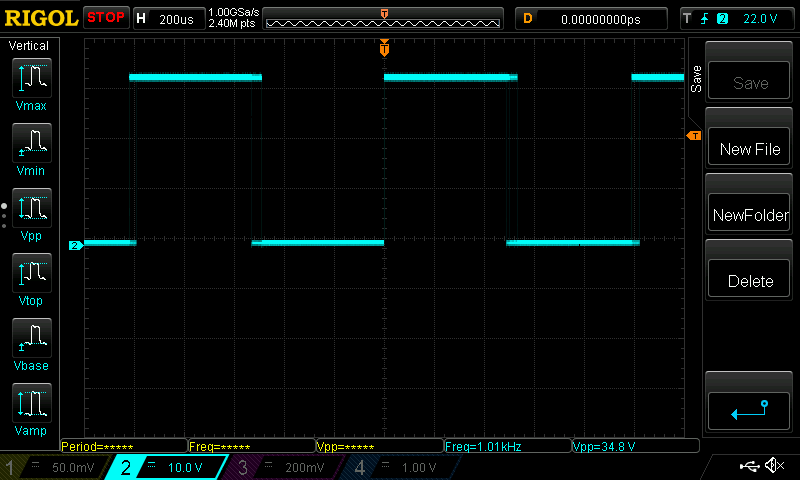
\includegraphics[scale = 0.5]{NewFile1.png}
	\caption{the generated waveform with the disturbance}
\end{figure}

\section{1.1 Using a switch to toggle the LED, Low Level Approach}
Following the instructions in the Lab7document we created an empty project in SWB4STM32, than the pointers for the GPIOA\_MODER, GPIOA\_ODR, GPIOC\_MOER, GPIOC\_IDR and RCC\_AHB1ENR have been initialized. \\
The clock has been configured to 1 for the GPIOA and GPIOC devices, after that the GPIOA pin5 has been configured as output and GPIOC pin 13 as input.\\
The application code starts with the initialization of the led to $off$ than we acquire a first time the complemented value of the button in button\_old. In the infinite while loop as first time we acquire the complemented button's value in button, after we if a 0-1 transition happened we complement the bit 5 of GPIO\_ODR. As last action we update button\_old with the value button.


\section{Using a switch to toggle the LED, CubeMX approach}
In this section we'll deal with the same exercise as the previous one, using a CubeMX approach with LL (Low Layer) libraries. 

In CubeMX we set the GPIO input and output respectively to pin A5 and C13 to correctly configure the LED and Button.

Apart from the I/O configuration, the algorithm is implemented as the point 1.1.

	\begin{figure}[!h]
		\centering
		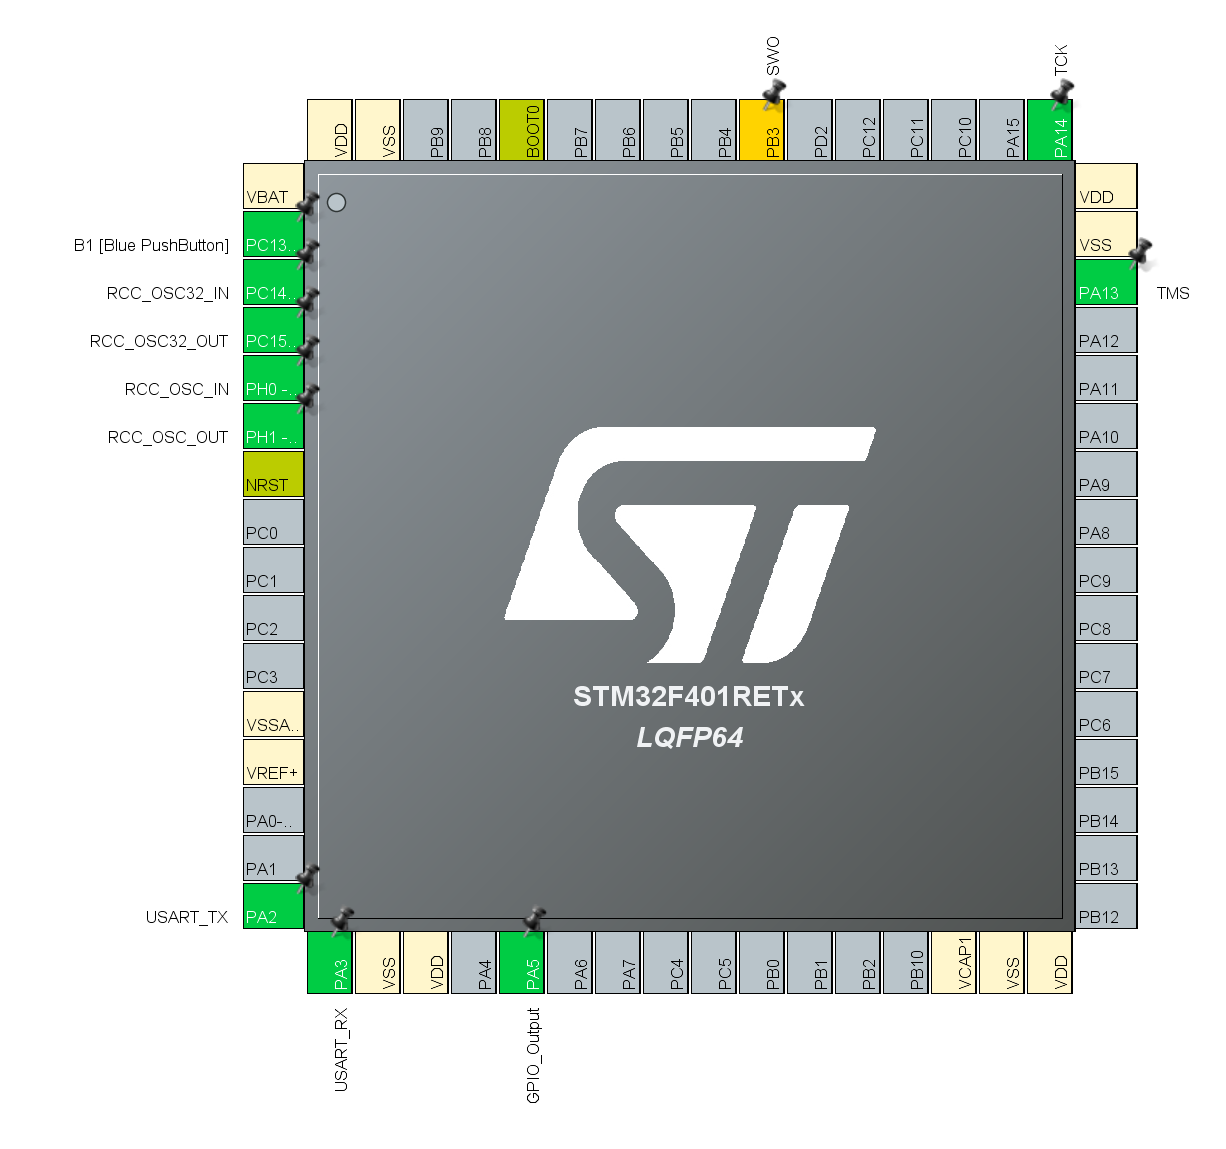
\includegraphics[scale = 0.7]{immagini/1_2.png}
		\caption{CubeMX GPIO configurations}
	\end{figure}

\section{Varying the blinking frequency}

Varying the maximum "for" counting number we can play on the blinking frequency.
The maximum appreciable frequency is around , due to 2 main reasons:
The maximal frame rate humans can perceive is around 70 Hz. Furthermore the LED being not an ideal component shows parasitic effects (Equivalent RC filter) that decrease the maximum appreciable frequency to about 60 Hz. 




>>>>>>> master

\end{document}




